% =====================================================================
% Explainable knowledge-tracing-based adaptive learning framework
% Compile: pdflatex main.tex (twice). For an IEEE journal template,
% replace the documentclass with \documentclass[journal]{IEEEtran}.
% Every number in tables/*.tex is produced by make_tables.py from the
% result CSV files; red [fill] marks a value that must still be inserted.
% =====================================================================
\documentclass[11pt]{article}
\usepackage[a4paper,margin=2.2cm]{geometry}

\IfFileExists{lmodern.sty}{\usepackage[T1]{fontenc}\usepackage{lmodern}}{}
\usepackage{amsmath,amssymb}
\usepackage{graphicx}
\usepackage{booktabs}
\usepackage{multirow}
\usepackage{tabularx}
\usepackage{array}
\usepackage{xcolor}
\usepackage{listings}
\usepackage{caption}
\usepackage{subcaption}
\usepackage{tikz}
\usetikzlibrary{positioning,arrows.meta,fit,backgrounds}
\usepackage[hidelinks]{hyperref}
\usepackage{cite}

\captionsetup{labelfont=normalfont,textfont=normalfont,font=small,labelsep=period}
\captionsetup[figure]{name=Fig.}
\captionsetup[table]{name=Table}
\renewcommand{\lstlistingname}{Algorithm}
\renewcommand{\thesubfigure}{\alph{subfigure}}

\makeatletter\newcommand{\tabin}[1]{\@@input #1 }\makeatother
\newcommand{\TBD}{\textcolor{red}{[fill]}}
\newcommand{\figfile}[2][\linewidth]{%
  \IfFileExists{figures/#2.png}{\includegraphics[width=#1]{figures/#2.png}}%
  {\fbox{\parbox[c][0.45\linewidth][c]{0.92\linewidth}{\centering\small\textcolor{red}{copy figures/\detokenize{#2}.png}}}}}

\definecolor{codegray}{gray}{0.45}
\lstset{
  language=Python,
  basicstyle=\ttfamily\footnotesize,
  keywordstyle=\color{blue!60!black},
  commentstyle=\color{codegray},
  stringstyle=\color{green!35!black},
  numbers=left, numberstyle=\tiny\color{codegray}, numbersep=6pt,
  frame=tb, framerule=0.4pt, breaklines=true, columns=fullflexible,
  captionpos=t, abovecaptionskip=4pt, xleftmargin=1.5em, showstringspaces=false
}

\title{An Explainable Knowledge-Tracing-Based Adaptive Learning Framework for Personalized Pedagogical Recommendation}
\author{Ayesha Kalsoom\\
\small Department of \TBD\\ \small National University of Computer and Emerging Sciences (FAST-NUCES), Islamabad, Pakistan\\
\small i257805@isb.nu.edu.pk}
\date{}

\begin{document}
\maketitle

% ---------------------------------------------------------------------
\begin{abstract}
Adaptive learning systems commonly use knowledge tracing (KT) to estimate what a learner knows and to decide which item the learner should practice next, but they rarely decide how the next learning step should be taught, and the few systems that recommend instruction seldom justify their recommendations. This paper presents an explainable KT-based framework that predicts the correctness of a learner's next response and converts the predicted learner state into a ranked list of five pedagogical strategies, namely remedial learning, example-based learning, practice-heavy learning, step-by-step guidance, and challenge-based learning, together with a feature-level explanation of each recommendation. The prediction component combines a strictly causal learner state, which contains a behavioral profile, pre-response context features, and an online difficulty-adjusted mastery estimate inspired by the Elo rating system, with a behavior-aware sequence network in which a gated cross-attention block fuses the encoded interaction history with the representation of the target question. The sequence backbone and the input groups are selected on validation learners only, and the recommendation component is trained on the strategies that are relevant at the learner's next step and is explained with SHapley Additive exPlanations (SHAP). The framework was evaluated on EdNet-KT3 and on ASSISTments 2017 under a learner-disjoint 70/10/20 split, with three random seeds, a paired learner-level bootstrap test, leave-one-group-out ablations, and explicit target-leakage checks. On EdNet-KT3, the proposed model reached a test area under the receiver operating characteristic curve (AUC) of 0.7742 $\pm$ 0.0003, whereas a controlled adaptation of the hierarchical graph attention knowledge tracing and personalized recommendation (HGAKT+PR) base model reached 0.7587 and attentive knowledge tracing (AKT) reached 0.7566. On ASSISTments 2017, the proposed model reached a test AUC of 0.8481 $\pm$ 0.0002, whereas the HGAKT adaptation reached 0.8131 and deep knowledge tracing (DKT) reached 0.7943, and every AUC improvement over every baseline was significant at $p \leq 0.001$. These results show that a causal and difficulty-aware learner state, when it is fused with sequence attention and selected without any use of the test set, yields a more accurate and more transparent basis for recommending how a learner should be taught.
\end{abstract}

\noindent\textit{Keywords:} knowledge tracing, adaptive learning, pedagogical recommendation, explainable artificial intelligence, learner modeling, EdNet, ASSISTments.

% ---------------------------------------------------------------------
\section{Introduction}

Online learning platforms, intelligent tutoring systems (ITSs), and massive open online courses (MOOCs) now record millions of learner interactions every day, and this scale has made data-driven personalization a central goal of educational technology. Knowledge tracing (KT) is the task of estimating a learner's evolving knowledge state from the sequence of past interactions and of predicting whether the learner will answer the next question correctly, and a recent survey has shown that KT has become the core learner-modeling component of most adaptive learning systems \cite{shen2024survey}. The practical value of KT, however, does not lie in the prediction itself but in the decision that the prediction supports, and most existing systems use the predicted knowledge state to answer a single question, namely what the learner should study next. The literature on accessible and inclusive online education has emphasized that learners differ not only in what they know but also in how they need to be supported, because a learner who repeatedly fails a concept needs a different form of instruction from a learner who has already mastered it \cite{lomellini2025accessible}. A second and equally important question, namely how the next learning step should be taught, has therefore received far less attention than item selection, although it determines whether a learner receives a worked example, step-by-step guidance, additional practice, remedial review, or a more challenging task. The rapid adoption of generative artificial intelligence in education has further increased the demand for systems that can adapt instruction rather than only content, while it has also increased the demand for transparent decisions that teachers can inspect \cite{denny2024computing}. An adaptive recommendation that cannot be explained is difficult for a teacher to trust, and the design of trustworthy KT models has consequently become an explicit research objective in its own right \cite{lu2024design}. Fig.~\ref{fig:motivation} contrasts the question that existing KT-based systems answer with the question that the present work addresses.

\begin{figure}[t]
\centering
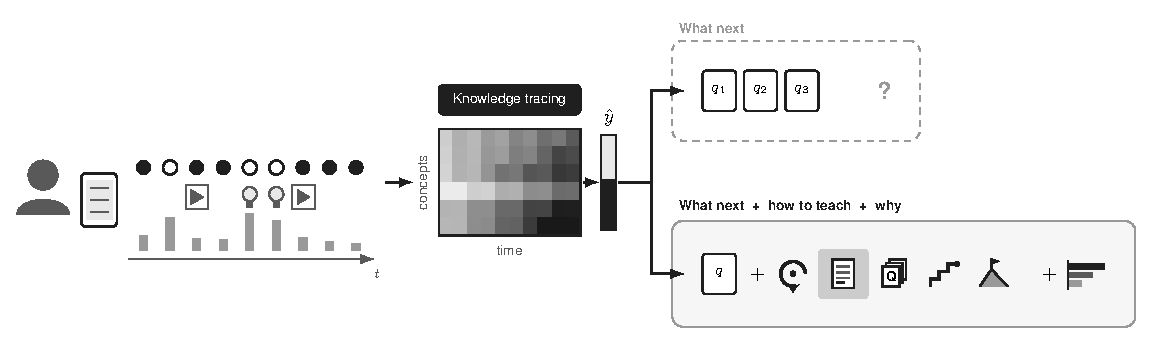
\includegraphics[width=\linewidth]{figures/arch_intro.pdf}
\caption{Conventional KT-based systems turn the predicted knowledge state into a choice of what a learner should study next, whereas the proposed framework also recommends how the next step should be taught through one of five pedagogical strategies and explains why.}
\label{fig:motivation}
\end{figure}


The base model of this study is the hierarchical graph attention knowledge tracing and personalized recommendation (HGAKT+PR) framework, which models a chapter, concept, and sub-concept hierarchy with multi-head graph attention and a dynamic gate and which jointly optimizes answer prediction and the recommendation of learning resources \cite{chen2026hierarchical}. HGAKT+PR represents an important step towards the integration of prediction and recommendation, but it recommends items rather than instructional strategies, it relies on a curriculum hierarchy that is not available in every dataset, and it does not explain why a particular recommendation was produced. A recent behavior-aware model has shown that pre-class and in-class behaviors carry information that response sequences alone do not contain, and it has also reported that EdNet remains a difficult benchmark on which the area under the receiver operating characteristic curve (AUC) of strong models remains close to 0.75 \cite{wang2026knowledge}. These observations motivate the central idea of the present work, which is that the behavioral and contextual information recorded by a platform should be converted into a strictly causal learner state, that this state should be fused with sequence attention for prediction, and that the same state should then drive an explainable recommendation of how the learner should be taught. The research problem is therefore formulated in two coupled parts: the first part concerns the accurate and leakage-free prediction of the next response from rich behavioral logs, and the second part concerns the conversion of the predicted learner state into a ranked and explainable list of pedagogical strategies.

This study makes four contributions. First, it proposes a behavior-aware KT network that combines a causal learner profile, twenty pre-response context features, an online difficulty-adjusted mastery estimate in the spirit of the Elo rating system, and question metadata embeddings with a causal Transformer history encoder and a gated cross-attention fusion block, and it shows that every input is computed from information that is available before the learner answers. Second, it introduces a validation-only selection protocol that chooses the sequence backbone and the input groups for each dataset without any access to the test learners, so that the reported test results are not the product of test-set tuning. Third, it proposes a pedagogical recommender that is trained on the strategies that are relevant at the learner's next step instead of the strategy that a rule assigns to the current step, which removes the circularity that arises when a classifier is evaluated against the same rule that generated its training labels, and it explains every recommendation with SHapley Additive exPlanations (SHAP). Fourth, it presents a rigorous evaluation on EdNet-KT3 and ASSISTments 2017 that includes eleven prediction baselines, a controlled adaptation of the HGAKT+PR base model, three random seeds, a paired learner-level bootstrap test, leave-one-group-out ablations with confidence intervals, a stepwise construction study, training-stability checks, and target-leakage tests.

The remainder of this paper is organized as follows. Section~\ref{sec:related} reviews related work on KT, graph-based and behavior-aware learner modeling, explainable KT, and educational recommendation. Section~\ref{sec:problem} formulates the problem and defines the notation. Section~\ref{sec:method} describes the proposed framework, and Section~\ref{sec:setup} describes the datasets, baselines, and evaluation protocol. Section~\ref{sec:results} reports and analyses the results, Section~\ref{sec:discussion} discusses their implications and the scope of the evidence, and Section~\ref{sec:conclusion} concludes the paper.

% ---------------------------------------------------------------------
\section{Related Work}\label{sec:related}

\subsection{Deep and Attention-Based Knowledge Tracing}

Deep KT models replace hand-crafted learner models with neural sequence encoders, and attention-based models have become the dominant family because attention can relate the current question directly to the most relevant past interactions. Enhancing locality for attentive knowledge tracing (ELAKT) showed that standard self-attention underweights the most recent interactions and that an explicit locality bias improves attentive KT \cite{pu2024elakt}. A self-attentive convolutional model has similarly combined convolution and attention to capture short-range and long-range dependencies in response sequences \cite{kia2024ackt}. A multi-layer attention KT method with self-supervised noise tolerance has further shown that attention models are sensitive to noisy responses such as guesses and slips \cite{wang2025multilayer}. Data sparsity remains a fundamental limitation of these models, because most learners answer only a small fraction of the available questions, and quantum-computing-enhanced KT has been proposed specifically to mitigate this sparsity \cite{bao2024quantum}. Adaptive time convolution with discrete cosine transform attention has also been used to model the temporal rhythm of learning more faithfully than position embeddings alone \cite{wang2025datckt}. These studies demonstrate that attention architectures continue to improve, but they mainly operate on the identity of the question and the correctness of the response, and they make little use of the behavioral context that modern platforms record.

\subsection{Graph-Based and Hierarchical Knowledge Tracing}

Graph-based KT models represent the relations between questions, concepts, and learners as graphs and propagate knowledge along these relations. Dynamic graph learning for knowledge tracing (DyGKT) treats the growing interaction record as a continuously evolving graph and updates learner and question representations over time \cite{cheng2024dygkt}. Temporal graph memory networks have extended this direction by storing the temporal evolution of the knowledge state in a graph memory \cite{gad2026temporal}. An information-processing dynamic graph has also been proposed to model the way in which learners process information during practice \cite{xiao2026information}. Long-term and short-term knowledge state graphs with adaptive fusion have shown that a learner's stable knowledge and transient state should be modelled separately \cite{yu2025exploring}. Hierarchical heterogeneous graphs have been used to represent the multi-level organization of course content \cite{li2026hierarchical}. Multi-association heterogeneous graph embedding has exploited knowledge transfer between related concepts \cite{yang2025mahkt}. Graph KT has also been used to test classic assertions of cognitive psychology in realistic cognitive situations \cite{wu2025graph}. Dual graph convolutional networks with positive and negative feature enhancement have been proposed to separate the evidence provided by correct and incorrect responses \cite{wang2025dual}. HGAKT+PR belongs to this family, and its chapter, concept, and sub-concept hierarchy is the main structural assumption that distinguishes it from flat graph models. The present work does not reject graph modeling, but it tests whether a richer causal learner state can provide a larger gain than additional graph structure when the curriculum hierarchy must be approximated from the available metadata.

\subsection{Behavior-Aware Knowledge Tracing}

Behavior-aware KT models add information about how a learner interacts with the platform in addition to whether the learner answers correctly. Integrating question information with learning behavior has been shown to improve KT on several public datasets \cite{su2025integrate}. Multi-task modeling of student knowledge and behavior has demonstrated that predicting the next behavior together with the next response improves the learned representation \cite{zhao2024multitask}. Time-frequency coupling with learning-behavior decoupling has further separated the behavioral signal from the knowledge signal in order to reduce their mutual interference \cite{huang2026timefrequency}. Classroom engagement and temporal-spatial features have been fused with KT in blended classrooms \cite{shou2024research}. Psychological factors have been added to heterogeneous learning-interaction graphs in order to model the learning process more completely \cite{wang2024psychological}. These studies support the premise of the present work, but they rarely state whether every behavioral feature is computed causally, and a behavior statistic that includes the current response introduces target leakage that can inflate the reported accuracy. The present framework therefore computes every learner-state variable from previous interactions only and verifies this property with an explicit leakage test.

\subsection{Explainable Knowledge Tracing}

Explainability has become a major research direction in KT because a prediction that cannot be inspected is difficult to use in instruction. A recent survey has organized explainable KT methods into static and temporal explanation methods and has documented their applications \cite{li2025survey}. The explainable knowledge tracing (XKT) model has embedded cognitive learning theories into the model for questions that involve multiple knowledge concepts \cite{huang2024xkt}. Cognitive assimilation has been combined with item response theory (IRT) to obtain a deep KT model whose parameters have a psychometric meaning \cite{guo2025deep}. Fine-grained multi-feature attribution has been used to explain which input features drive each prediction \cite{liang2026interpretable}. Theory-based interpretability has been introduced into deep KT through grounded Transformers \cite{labra2026theory}. Elo-based learning systems provide an additional transparent family of learner models, and recent psychometric work has evaluated and improved the measurement properties of Elo ratings in learning systems \cite{bolsinova2025keeping}. Outside KT, explainable machine learning models with SHAP have been used to explain the prediction of student scores in tertiary education \cite{ghimire2024explainable}. The present work draws on these directions in two ways: it uses an online difficulty-adjusted mastery estimate whose values have a direct interpretation, and it explains the pedagogical recommendation, rather than only the prediction, with SHAP attributions.

\subsection{Recommendation in Adaptive Learning}

Educational recommendation has mainly focused on the selection of exercises, resources, or learning paths. Learning-path recommendation with multi-behavior user modeling and cascading deep Q-networks has optimized the order of learning activities with reinforcement learning \cite{ma2024learning}. Personalized exercise recommendation with semantically grounded KT has linked the KT state to the semantic content of exercises \cite{ozyurt2025personalized}. Heterogeneous knowledge graph attention has been used to produce explainable recommendations in a general recommender setting \cite{zhang2025hkgat}. Language models have been combined with KT for personalized question generation \cite{yin2025leveraging}. Optimal KT has been formulated for artificial-intelligence-assisted personalized programming education \cite{wang2026futureproofing}. These systems recommend what a learner should do next, whereas the present framework recommends how the next step should be taught. This distinction has an important methodological consequence, because the recommendation targets of item recommenders and strategy recommenders are different, so their ranking metrics cannot be compared directly, and the present work therefore compares prediction quality under a common protocol and evaluates strategy recommendation against its own relevance definition.

% ---------------------------------------------------------------------
\section{Problem Formulation}\label{sec:problem}

Table~\ref{tab:abbrev} lists every abbreviation that is used in this paper, and each abbreviation is also defined at its first use in the text. Let $\mathcal{U}$ denote the set of learners and let $\mathcal{Q}$ denote the set of questions. For a learner $u \in \mathcal{U}$, the interaction history up to step $t$ is the ordered sequence that is defined in (\ref{eq:history}), in which $q_i \in \mathcal{Q}$ is the question at step $i$, $r_i \in \{0,1\}$ indicates whether the response was correct, and $\mathbf{x}_i$ collects the behavioral and contextual observations that are attached to the interaction.
\begin{equation}\label{eq:history}
\mathcal{H}_t^{u} = \big((q_1, r_1, \mathbf{x}_1), (q_2, r_2, \mathbf{x}_2), \dots, (q_t, r_t, \mathbf{x}_t)\big).
\end{equation}
The prediction task is to estimate the probability that is defined in (\ref{eq:task}), where $\mathbf{s}_{t+1}$ is the learner state that is available immediately before the learner answers question $q_{t+1}$.
\begin{equation}\label{eq:task}
\hat{y}_{t+1} = P\big(r_{t+1} = 1 \mid \mathcal{H}_t^{u}, q_{t+1}, \mathbf{s}_{t+1}\big).
\end{equation}
The causality constraint requires that $\mathbf{s}_{t+1}$ must not depend on $r_{t+1}$, on the response time of step $t+1$, or on any later observation. The recommendation task is to produce, for every learner state, a ranking of the strategy set $\mathcal{S} = \{$remedial, example-based, practice-heavy, step-by-step, challenge-based$\}$ and to return the top-$K$ strategies together with the features that explain the ranking. Because the datasets do not contain randomized assignments of pedagogical strategies, the recommendation task is defined as the ranking of strategies that are relevant to the learner's next state, and it is not defined as the estimation of the causal effect of a strategy on learning.

\begin{table}[t]
\centering
\caption{Abbreviations used in this paper.}
\label{tab:abbrev}
\small
\begin{tabularx}{\linewidth}{@{}lX@{\hspace{1em}}lX@{}}
\toprule
Abbreviation & Meaning & Abbreviation & Meaning \\
\midrule
AdamW & Adam optimizer with decoupled weight decay & LSTM & Long short-term memory \\
AKT & Attentive knowledge tracing & MLP & Multilayer perceptron \\
AUC & Area under the receiver operating characteristic curve & MOOC & Massive open online course \\
CI & Confidence interval & NDCG@$K$ & Normalized discounted cumulative gain at rank $K$ \\
DKT & Deep knowledge tracing & P@$K$ & Precision at rank $K$ \\
DyGKT & Dynamic graph learning for knowledge tracing & R@$K$ & Recall at rank $K$ \\
ELAKT & Enhancing locality for attentive knowledge tracing & RMSE & Root mean squared error \\
F1 & Harmonic mean of precision and recall & ROC & Receiver operating characteristic \\
GELU & Gaussian error linear unit & SAINT+ & Separated self-attentive neural knowledge tracing with temporal features \\
GPU & Graphics processing unit & SAKT & Self-attentive knowledge tracing \\
HGAKT+PR & Hierarchical graph attention knowledge tracing and personalized recommendation & SHAP & SHapley Additive exPlanations \\
IRT & Item response theory & TOEIC & Test of English for International Communication \\
ITS & Intelligent tutoring system & XGBoost & Extreme gradient boosting \\
KT & Knowledge tracing & XKT & Explainable knowledge tracing \\
\bottomrule
\end{tabularx}
\end{table}

% ---------------------------------------------------------------------
\section{Proposed Framework}\label{sec:method}

\subsection{Overview}

Fig.~\ref{fig:framework} shows the overall framework, which processes each learner interaction in five stages. The first stage converts the raw interaction log into a strictly causal learner state, the second stage adds an online difficulty-adjusted mastery estimate, the third stage predicts the correctness of the next response with a behavior-aware sequence network, the fourth stage ranks the five pedagogical strategies from the predicted learner state, and the fifth stage explains each ranking with SHAP attributions. A validation-only selection protocol fixes the backbone and the input groups of the prediction network for each dataset before any test learner is evaluated, and the same protocol fixes the design and the class-balancing strength of the recommender.

\begin{figure}[t]
\centering
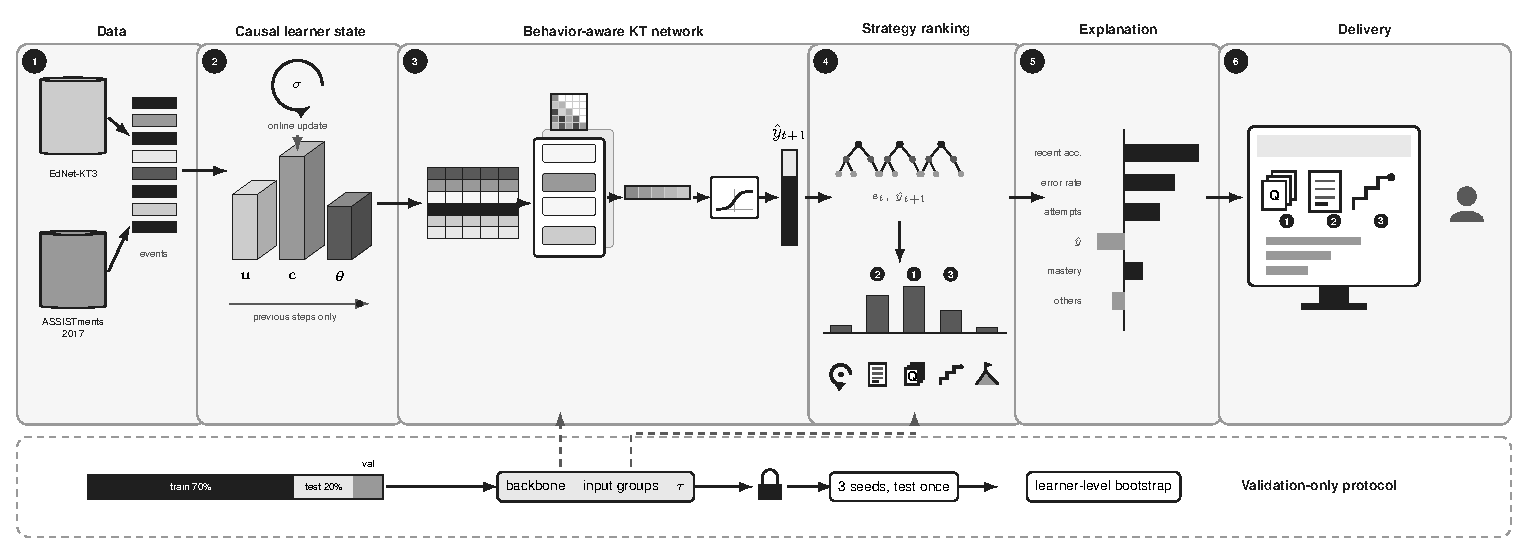
\includegraphics[width=\linewidth]{figures/arch_system.pdf}
\caption{Overall architecture of the proposed framework. The numbered panels show the data sources, the causal learner state, the behavior-aware KT network, the ranking of the five pedagogical strategies, the SHAP explanation, and the delivery of the recommendation, and the lower band shows the validation-only protocol that fixes the design before the test learners are evaluated once.}
\label{fig:framework}
\end{figure}

\subsection{Causal Learner State}

The learner state contains three groups of variables, and every variable is stored before the current response updates the state. The first group is the learner profile, which contains ten running statistics, namely historical accuracy, recent accuracy over the last ten responses, topic mastery, mean response time, mean number of attempts, explanation rate, mean explanation time, lecture rate, mean lecture time, and the rate at which adaptively offered content was accepted. The historical accuracy of learner $u$ at step $t$ is computed by (\ref{eq:histacc}), and the other running statistics follow the same prefix-only form.
\begin{equation}\label{eq:histacc}
a_t^{u} = \frac{1}{t-1}\sum_{i=1}^{t-1} r_i, \qquad t > 1 .
\end{equation}
An earlier audit of the feature set showed that the error rate is exactly $1-a_t^{u}$ and that the review rate is effectively constant, and both variables were therefore removed from the network input in order to avoid redundant and uninformative dimensions. The second group contains twenty pre-response context features that are organized into five groups. The experience group records whether the interaction is the learner's first interaction and how long the learner's history is. The timing group records the lag since the previous interaction, whether the question belongs to the same bundle as the previous question, the position of the question in its bundle, and the position of the interaction in the current session. The recency group records, for the same question and for the same skill, whether the learner has seen it before, how many attempts the learner has made, whether the last attempt was correct, and how much time has passed since the last attempt. The engagement group records whether the learner opened an explanation or a lecture since the previous question, together with the change in the count and in the time spent. The source and platform group embeds the platform and the content source from which the question was served. The third group contains the question metadata, namely the TOEIC part and the knowledge tags of each question in EdNet-KT3, or the skill tags in ASSISTments 2017. Fig.~\ref{fig:state} illustrates the order of operations at every step, in which the state is stored first, the learner answers second, and the state is updated only third, together with the difficulty-adjusted mastery loop that is described next.

\begin{figure}[t]
\centering
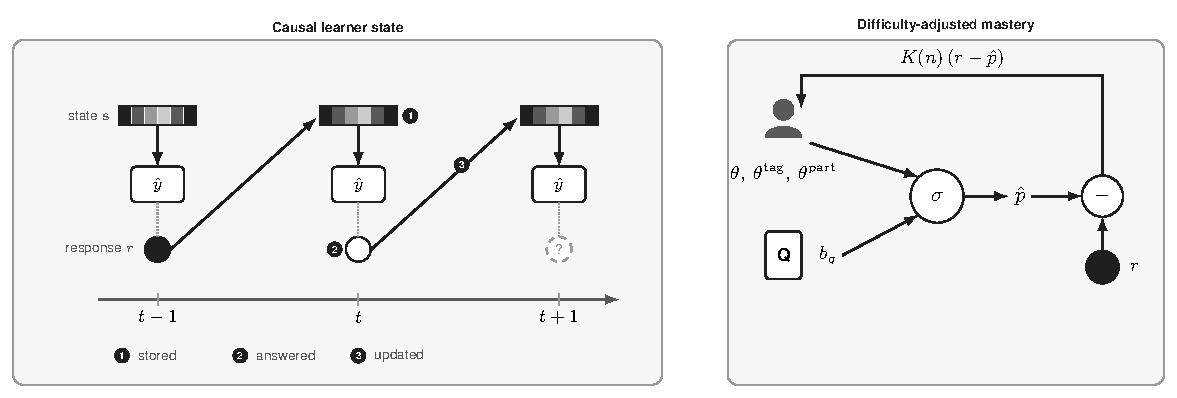
\includegraphics[width=\linewidth]{figures/fig_state.pdf}
\caption{Construction of the causal learner state (left) and of the online difficulty-adjusted mastery estimate (right). The response of a step updates only the state of the following step.}
\label{fig:state}
\end{figure}


\subsection{Online Difficulty-Adjusted Mastery}

Raw accuracy statistics ignore the difficulty of the answered questions, and on an adaptive platform stronger learners receive harder questions, so a raw percentage separates learners poorly. The framework therefore adds an online mastery estimate that is measured against question easiness. The easiness of question $q$ is estimated from training learners only by the smoothed logit in (\ref{eq:easiness}), where $h_q$ and $n_q$ are the number of correct responses and the number of responses to $q$, $\pi$ is the global training accuracy, and $\kappa = 20$ is the smoothing strength.
\begin{equation}\label{eq:easiness}
b_q = \log\frac{\tilde{p}_q}{1-\tilde{p}_q}, \qquad \tilde{p}_q = \frac{h_q + \kappa\,\pi}{n_q + \kappa}.
\end{equation}
Inside the training set, $b_q$ is computed out of fold over five learner folds, so that the easiness that is used for a training learner never contains that learner's own responses, while validation and test learners use the easiness that is computed from all training learners. The expected probability of a correct response is obtained by (\ref{eq:elo}), where $\theta_t$ is the global ability, $\bar{\theta}^{\text{tag}}_t$ is the mean ability over the question's knowledge tags, $\theta^{\text{part}}_t$ is the ability for the question's part, and $\sigma(\cdot)$ is the logistic function.
\begin{equation}\label{eq:elo}
\hat{p}^{\text{elo}}_t = \sigma\big(\theta_t + \bar{\theta}^{\text{tag}}_t + \theta^{\text{part}}_t + b_{q_t}\big).
\end{equation}
After the features of step $t$ have been stored, each ability is updated by the rule in (\ref{eq:eloupdate}), where $n$ is the number of previous updates of that ability and the constants $(\alpha,\delta,\epsilon)$ were fixed before any experiment to $(0.4, 0.05, 0.01)$ for the global ability, $(0.4, 0.10, 0.02)$ for the tag abilities, and $(0.3, 0.05, 0.01)$ for the part ability.
\begin{equation}\label{eq:eloupdate}
\theta \leftarrow \theta + \max\!\Big(\frac{\alpha}{1+\delta n},\, \epsilon\Big)\big(r_t - \hat{p}^{\text{elo}}_t\big).
\end{equation}
The mastery block contains nine values, namely the question easiness, the long-term ability, a short-term ability with a constant step size of 0.1, the mean and minimum tag abilities, the part ability, the expected probability, and the normalized practice counts for the tags and for the part. Algorithm~\ref{alg:elo} gives the complete causal computation, and its line order makes the leakage rule explicit, because the features of a row are written before the response of that row is used.

\begin{lstlisting}[caption={Causal computation of the difficulty-adjusted mastery features.},label={alg:elo}]
def mastery_features(items, correct, first, easiness, part_of, tags_of):
    out = np.zeros((len(items), 9), dtype=np.float32)
    for i in range(len(items)):
        if first[i]:                                   # new learner: reset the state
            ability, recent, seen = 0.0, 0.0, 0
            tag_ability, tag_seen = {}, {}
            part_ability, part_seen = [0.0] * 8, [0] * 8
        q, b = items[i], easiness[i]
        part, tags = part_of[q], tags_of[q]
        tag_vals = [tag_ability.get(g, 0.0) for g in tags] or [0.0]
        tag_mean, tag_min = np.mean(tag_vals), np.min(tag_vals)
        expected = sigmoid(ability + tag_mean + part_ability[part] + b)
        out[i] = [tanh(b / 2), tanh(ability / 2), tanh(recent / 2), tanh(tag_mean / 2),
                  tanh(tag_min / 2), tanh(part_ability[part] / 2), expected,
                  practice(tag_seen, tags), practice_part(part_seen[part])]
        # the response of row i is used only after its features were stored
        error = correct[i] - expected
        ability += max(0.4 / (1 + 0.05 * seen), 0.01) * error
        seen += 1
        recent += 0.1 * (correct[i] - sigmoid(recent + b))
        for g in tags:
            n = tag_seen.get(g, 0)
            tag_ability[g] = tag_ability.get(g, 0.0) + max(0.4 / (1 + 0.10 * n), 0.02) * error
            tag_seen[g] = n + 1
        part_ability[part] += max(0.3 / (1 + 0.05 * part_seen[part]), 0.01) * error
        part_seen[part] += 1
    return out
\end{lstlisting}

\subsection{Behavior-Aware Knowledge Tracing Network}

The network separates the representation of past interactions, whose responses are known, from the representation of the target question, whose response must be predicted. Fig.~\ref{fig:arch} shows the complete network, and the following equations define each of its components. Each history token is formed by (\ref{eq:histtoken}), where $\mathbf{e}^{s}$, $\mathbf{e}^{q}$, and $\mathbf{e}^{r}$ are the skill, question, and response embeddings, $\mathbf{p}_i$ is the position embedding, $\phi_b$, $\phi_\tau$, and $\phi_c$ are projections of the behavioral profile, the elapsed time and lag, and the context vector, $\mathbf{m}_i$ is the sum of the source, platform, part, and mean tag embeddings, $\odot$ denotes the element-wise product, and $F_h$ is a two-layer fusion network with a Gaussian error linear unit (GELU) and layer normalization.
\begin{equation}\label{eq:histtoken}
\mathbf{h}_i = F_h\big([\mathbf{e}^{s}_{i};\, \mathbf{e}^{q}_{i};\, \mathbf{e}^{r}_{i};\, \mathbf{p}_i;\, \phi_b(\mathbf{b}_i);\, \phi_\tau(\Delta_i);\, \mathbf{e}^{s}_{i}\odot\mathbf{e}^{q}_{i};\, \phi_c(\mathbf{c}_i);\, \mathbf{m}_i]\big).
\end{equation}
The target query for step $t+1$ is formed by (\ref{eq:query}) from information that is available before the response, where $\phi_u$ projects the learner profile $\mathbf{u}_{t+1}$ and $F_z$ is a second fusion network, and the query therefore contains no response embedding and no response time of the target step.
\begin{equation}\label{eq:query}
\mathbf{z}_{t+1} = F_z\big([\mathbf{e}^{s}_{t+1};\, \mathbf{e}^{q}_{t+1};\, \mathbf{p}_{t+1};\, \phi_u(\mathbf{u}_{t+1});\, \mathbf{e}^{s}_{t+1}\odot\mathbf{e}^{q}_{t+1};\, \phi_c(\mathbf{c}_{t+1});\, \mathbf{m}_{t+1}]\big).
\end{equation}
The history tokens are encoded by a causal pre-normalized Transformer encoder, and the target query attends to the encoded history through multi-head cross-attention, as written in (\ref{eq:attn}), where the causal mask restricts the query of step $t+1$ to history tokens $1,\dots,t$.
\begin{equation}\label{eq:attn}
\mathbf{H} = \mathrm{Enc}_{\text{causal}}(\mathbf{h}_{1:t}), \qquad \mathbf{a}_{t+1} = \mathrm{MHA}\big(\mathbf{z}_{t+1}, \mathbf{H}, \mathbf{H}\big).
\end{equation}
A learned gate decides, for every dimension, how much the prediction should rely on the retrieved history and how much it should rely on the target representation, and the gate and the fused vector are computed by (\ref{eq:gate}), where $\mathrm{LN}$ denotes layer normalization.
\begin{equation}\label{eq:gate}
\mathbf{g} = \sigma\big(\mathbf{W}_g[\mathbf{z}_{t+1};\, \mathbf{a}_{t+1};\, \phi_u(\mathbf{u}_{t+1})]\big), \qquad \mathbf{f}_{t+1} = \mathrm{LN}\big(\mathbf{g}\odot\mathbf{a}_{t+1} + (1-\mathbf{g})\odot\mathbf{z}_{t+1}\big).
\end{equation}
The final probability combines a deep multilayer perceptron (MLP), a wide linear term over the raw profile and context values, and a question bias $\beta_{q}$, as defined in (\ref{eq:output}). The wide term gives the network direct access to well-calibrated numerical signals such as the expected Elo probability, and the question bias captures residual question difficulty.
\begin{equation}\label{eq:output}
\hat{y}_{t+1} = \sigma\Big(\mathrm{MLP}\big([\mathbf{f}_{t+1};\, \mathbf{z}_{t+1};\, \mathbf{a}_{t+1};\, \phi_u(\mathbf{u}_{t+1});\, \phi_c(\mathbf{c}_{t+1})]\big) + \mathbf{w}^{\top}[\mathbf{u}_{t+1};\, \mathbf{c}_{t+1}] + \beta_{q_{t+1}}\Big).
\end{equation}
The network is trained by minimizing the binary cross-entropy in (\ref{eq:loss}) over all eligible target steps $\mathcal{T}$, where a step is eligible when the learner has at least five previous interactions.
\begin{equation}\label{eq:loss}
\mathcal{L}_{\text{KT}} = -\frac{1}{|\mathcal{T}|}\sum_{(u,t)\in\mathcal{T}} \Big[r_{t}^{u}\log\hat{y}_{t}^{u} + (1-r_{t}^{u})\log\big(1-\hat{y}_{t}^{u}\big)\Big].
\end{equation}
The same network can be instantiated with a long short-term memory (LSTM) backbone, in which an LSTM replaces the Transformer history encoder and the last hidden state replaces the cross-attention output, and this alternative is one of the candidates of the selection protocol.

\begin{figure*}[t]
\centering
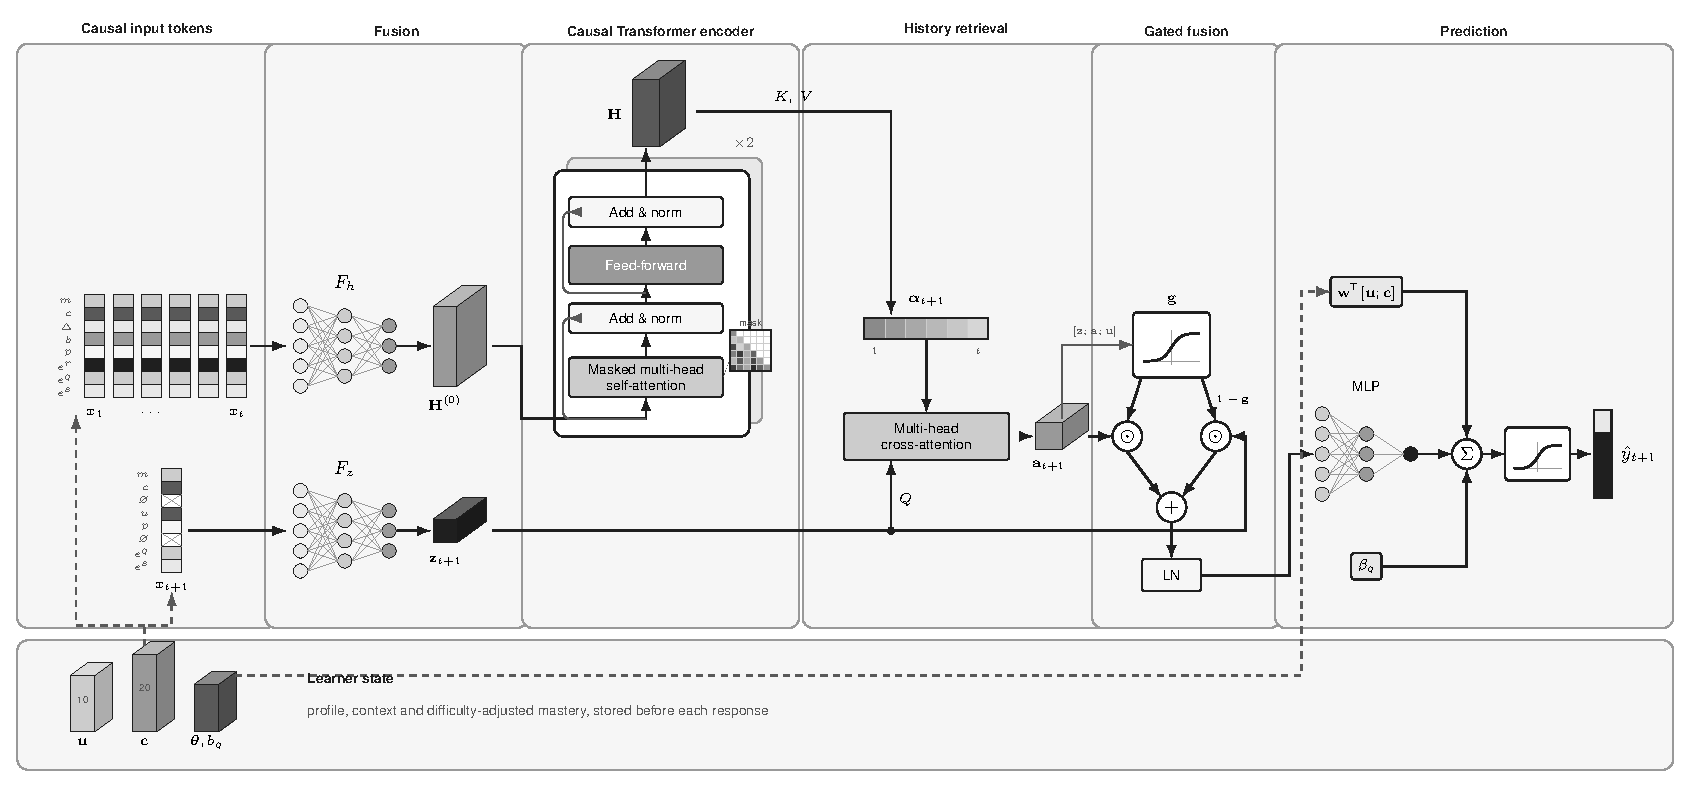
\includegraphics[width=\linewidth]{figures/arch_model.pdf}
\caption{Architecture of the behavior-aware KT network. Each history token stacks the skill ($e^{s}$), question ($e^{q}$), response ($e^{r}$), position ($p$), behavior ($b$), timing ($\Delta$), context ($c$), and metadata ($m$) components, whereas the target token replaces the response and timing components, which are unavailable before the answer, with the learner profile ($u$). The masked encoder and the cross-attention restrict the target query to earlier interactions, the gate $\mathbf{g}$ fuses the retrieved history with the target representation, and the prediction combines a deep MLP, a wide linear term, and a question bias.}
\label{fig:arch}
\end{figure*}

\subsection{Validation-Only Design Selection}

A single fixed design is not necessarily the best design for every dataset, because datasets differ in sequence length, in the richness of their behavioral logs, and in the amount of data. The framework therefore selects the backbone and the input groups on validation learners with the rule in Algorithm~\ref{alg:select}. The backbone is chosen first by validation AUC, and each input group is then removed in turn and is discarded only when its removal does not lower the validation AUC. The test learners are not accessed during this procedure, and the selected configuration is subsequently trained with three random seeds and evaluated on the test learners once.

\begin{lstlisting}[caption={Validation-only selection of the backbone and the input groups.},label={alg:select}]
GROUPS = ["learner_profile", "recency", "experience_timing", "hint_context",
          "source_platform", "mastery_tags", "response_time", "recent_accuracy"]

def select_design(train, val, seed=42):
    scores = {bb: fit(train, val, backbone=bb, drop=[], seed=seed).val_auc
              for bb in ("attention", "lstm")}
    backbone = max(scores, key=scores.get)
    full_auc = scores[backbone]
    removed = []
    for group in GROUPS:                     # leave one group out, validation only
        auc = fit(train, val, backbone=backbone, drop=[group], seed=seed).val_auc
        if auc >= full_auc:                  # the group did not help on validation
            removed.append(group)
    if removed:
        final_auc = fit(train, val, backbone=backbone, drop=removed, seed=seed).val_auc
        if final_auc < full_auc:
            removed = []
    return backbone, removed                 # frozen before any test evaluation

def final_runs(train, val, test, backbone, removed, seeds=(42, 52, 62)):
    models = [fit(train, val, backbone=backbone, drop=removed, seed=s) for s in seeds]
    return [m.evaluate(test) for m in models]    # the test set is used once
\end{lstlisting}

\subsection{Pedagogical Strategy Recommendation}

The datasets do not contain an expert label that states which strategy should be used at each step, so the framework uses a transparent weak-supervision policy that maps the learner state to strategies. The policy uses the topic mastery $m$, the recent accuracy $\rho$, the mean number of attempts $\nu$, the error rate $e$, and the KT probability $\hat{y}$, and it declares a strategy relevant when the conditions in (\ref{eq:policy}) hold, where practice-heavy learning is also used as the default when no other condition holds.
\begin{equation}\label{eq:policy}
\begin{aligned}
\text{challenge} &: m \geq 0.80 \,\wedge\, \rho \geq 0.80 \,\wedge\, \hat{y} \geq 0.75,\\
\text{remedial} &: m < 0.35 \,\wedge\, \rho < 0.50 \,\wedge\, \hat{y} < 0.50,\\
\text{example-based} &: m < 0.55 \,\vee\, \hat{y} < 0.55,\\
\text{step-by-step} &: e \geq 0.45 \,\vee\, \nu \geq 1.50,\\
\text{practice-heavy} &: 0.50 \leq \rho < 0.80 \,\vee\, 0.50 \leq \hat{y} < 0.75 .
\end{aligned}
\end{equation}
An earlier version of the recommender was trained to reproduce the single strategy that the policy assigned to the current state and was evaluated against the same policy, and it reached a top-1 agreement of 0.9985. This agreement only shows that a classifier can learn a deterministic rule from the inputs of that rule, and it is not evidence of recommendation quality, so it is not reported as an effectiveness result in this paper. The proposed recommender instead learns the set of strategies that are relevant at the learner's next step, which is defined in (\ref{eq:relevance}) by applying the policy to the next learner state $\mathbf{s}^{u}_{t+1}$.
\begin{equation}\label{eq:relevance}
\mathcal{R}_t^{u} = \big\{\, s \in \mathcal{S} \;:\; \text{the condition of } s \text{ in (\ref{eq:policy}) holds for } \mathbf{s}^{u}_{t+1} \,\big\}.
\end{equation}
Fig.~\ref{fig:recommender} summarizes the three parts of the recommender, namely the next-step target, the class-balanced training, and the ranking with its explanation. Each pair of a current learner state and a relevant next-step strategy forms one training example of a gradient-boosted tree classifier based on extreme gradient boosting (XGBoost), so every rank of the returned list is trained rather than only the first rank. Because some strategies, in particular remedial and challenge-based learning, are rare, each training pair of strategy $s$ is weighted by (\ref{eq:balance}), where $\pi_s$ is the share of training pairs with strategy $s$ and $\tau \geq 0$ controls the strength of class balancing.
\begin{equation}\label{eq:balance}
w_s = \frac{\pi_s^{-\tau}}{\sum_{s'\in\mathcal{S}} \pi_{s'}\,\pi_{s'}^{-\tau}} .
\end{equation}
The value of $\tau$ and the input design of the recommender are selected on held-out validation learners, as shown in Algorithm~\ref{alg:recommend}. The recommender is fitted on 80\% of the validation learners, early stopping uses the remaining 20\%, and the evaluation uses the test learners, so the KT model has never been trained on any learner that is used to fit or to evaluate the recommender.

\begin{lstlisting}[caption={Training of the next-step pedagogical recommender with validation-selected class balancing.},label={alg:recommend}]
STRATEGIES = ["challenge", "example", "practice", "remedial", "step_by_step"]

def next_step_pairs(frame):
    nxt = frame.groupby("user_id")[STATE].shift(-1)          # next learner state
    rel = apply_policy(nxt)                                   # equation (13), multi-label
    rows, cols = np.nonzero(rel[frame.has_next])
    return frame.loc[frame.has_next, FEATURES].iloc[rows], cols

def fit_recommender(fit_users, stop_users, tau):
    x, y = next_step_pairs(fit_users)
    share = np.bincount(y, minlength=5) / len(y)
    w = share[y] ** (-tau)
    w = w / np.mean(w)                                        # equation (15)
    model = XGBClassifier(objective="multi:softprob", n_estimators=800, max_depth=6,
                          learning_rate=0.05, early_stopping_rounds=40)
    xs, ys = next_step_pairs(stop_users)
    return model.fit(x, y, sample_weight=w, eval_set=[(xs, ys)])

def select_recommender(fit_users, stop_users, designs, taus):
    best = None
    for design in designs:
        for tau in taus:
            model = fit_recommender(fit_users[design], stop_users[design], tau)
            score = ndcg_at_k(model, stop_users[design], k=3)   # validation only
            if best is None or score > best[0]:
                best = (score, design, tau, model)
    return best                                               # then evaluated once on test
\end{lstlisting}

\begin{figure}[t]
\centering
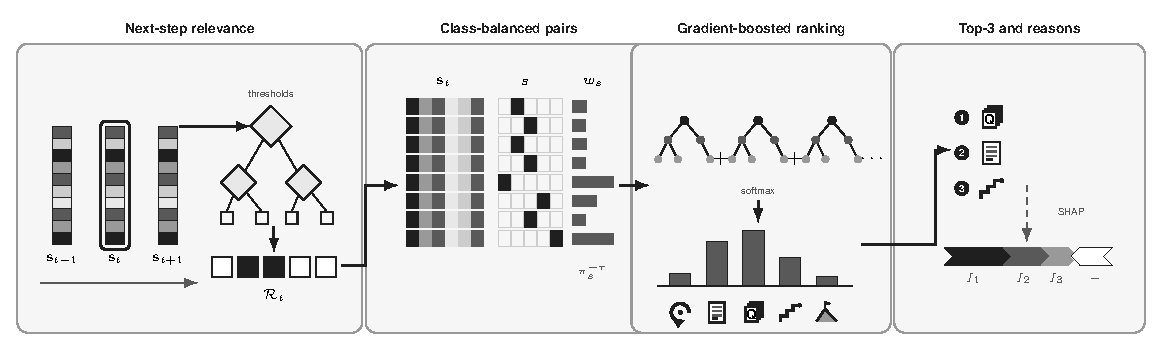
\includegraphics[width=\linewidth]{figures/arch_recommender.pdf}
\caption{Next-step pedagogical recommender. The threshold rule marks the strategies that are relevant at the next learner state, every relevant strategy forms a weighted training pair, gradient-boosted trees produce a probability for each strategy, and the top-3 strategies are returned with their SHAP reasons.}
\label{fig:recommender}
\end{figure}

The returned ranking is evaluated with precision, recall, normalized discounted cumulative gain, and hit rate at rank $K$. For a learner state with relevant set $\mathcal{R}$ and ranked list $L_K$, precision at rank $K$ (P@$K$) and recall at rank $K$ (R@$K$) are computed by (\ref{eq:pr}).
\begin{equation}\label{eq:pr}
\text{P@}K = \frac{|L_K \cap \mathcal{R}|}{K}, \qquad \text{R@}K = \frac{|L_K \cap \mathcal{R}|}{|\mathcal{R}|}.
\end{equation}
The normalized discounted cumulative gain at rank $K$ (NDCG@$K$) rewards relevant strategies that are ranked early, and it is computed by (\ref{eq:ndcg}), where $\mathrm{rel}_j$ indicates whether the strategy at rank $j$ is relevant.
\begin{equation}\label{eq:ndcg}
\text{NDCG@}K = \frac{\sum_{j=1}^{K} \mathrm{rel}_j / \log_2(j+1)}{\sum_{j=1}^{\min(K,|\mathcal{R}|)} 1/\log_2(j+1)} .
\end{equation}

\subsection{Explanation of Recommendations}

Every recommendation is explained with tree-based SHAP values, which attribute the score of each strategy to the input features of the learner state. The explanation that is presented to a teacher consists of the three features with the largest attributions for the top-ranked strategy, for example a low difficulty-adjusted tag ability, a low KT probability, and a high mean number of attempts for a remedial recommendation. The quality of the explanations is measured by fidelity and by consistency. Fidelity is the mean drop in the probability of the top-ranked strategy when the three most important features of each explanation are replaced by their background values, as defined in (\ref{eq:fidelity}), where $\mathbf{x}_{\setminus k}$ denotes the input after this replacement and $s^{*}$ is the top-ranked strategy.
\begin{equation}\label{eq:fidelity}
\text{Fidelity} = \frac{1}{N}\sum_{n=1}^{N}\Big[P\big(s^{*}_n \mid \mathbf{x}_n\big) - P\big(s^{*}_n \mid \mathbf{x}_{n,\setminus k}\big)\Big].
\end{equation}
Consistency is the mean Jaccard overlap between the top-feature sets of explanations that are computed for the same sample with different background samples, so a high consistency means that the explanation is stable.

% ---------------------------------------------------------------------
\section{Experimental Setup}\label{sec:setup}

\subsection{Datasets and Split}

Table~\ref{tab:data} summarizes the two datasets. EdNet-KT3 was collected from a mobile TOEIC preparation platform, and it contains question responses together with lecture views, explanation views, and adaptive content offers, which makes it suitable for behavior-aware modeling. ASSISTments 2017 was collected from a mathematics tutoring platform, it contains 3,162 problems that are labelled with 102 skills, and its hint requests play the role that explanation views play in EdNet-KT3. Both datasets were split at the learner level into 70\% training, 10\% validation, and 20\% test learners, so no learner contributes interactions to more than one subset, and the EdNet-KT3 split was frozen in a single assignment file that was shared by every model. Long sequences were divided into windows of 201 interactions with a stride of 200, and the first interaction of each window reuses the last interaction of the previous window as context.

\begin{table}[t]
\centering
\caption{Statistics of the datasets after preprocessing.}
\label{tab:data}
\small
\begin{tabular}{@{}lcc@{}}
\toprule
Statistic & EdNet-KT3 & ASSISTments 2017 \\
\midrule
\tabin{tables/data.tex}
\bottomrule
\end{tabular}
\end{table}

\subsection{Baselines}

The proposed model was compared with eleven baselines. The classical baselines were logistic regression, random forest, and XGBoost on the original learner features, and an additional XGBoost model was trained on exactly the same inputs as the proposed network in order to separate the contribution of the inputs from the contribution of sequence modeling. The deep baselines were deep knowledge tracing (DKT), the Transformer-based KT model (Transformer-KT), self-attentive knowledge tracing (SAKT), separated self-attentive neural knowledge tracing with temporal features (SAINT+), and attentive knowledge tracing (AKT), which have been reviewed in a recent survey \cite{shen2024survey}. The base model was a controlled adaptation of HGAKT+PR, which used two graph attention layers with six heads, a dynamic gate, an LSTM predictor with 256 hidden units, a hierarchy that was approximated by part, tag, skill, and question relations, and a training-only question difficulty, as described by its authors \cite{chen2026hierarchical}. The HGAKT+PR paper does not disclose the hidden dimension, the batch size, the weight of the joint loss, or the code for the construction of the hierarchy, and these settings were therefore chosen as stated above and were kept fixed. All baselines used the same split, the same eligible target rows, and the same metrics, and the published HGAKT+PR results on EdNet-KT1 were not compared numerically with the present results, because they were obtained on a different dataset and with a different protocol.

\subsection{Implementation and Training}

Table~\ref{tab:hyper} lists the training settings, which differ between the datasets only in the batch size, the epoch limit, and the early-stopping patience, because ASSISTments 2017 contains far fewer learners than EdNet-KT3. All neural models were trained with the Adam optimizer with decoupled weight decay (AdamW), gradient clipping, and early stopping on the validation AUC, and the decision threshold for accuracy, precision, recall, and the F1-score was selected on the validation learners by maximizing the F1-score. The F1-score is the harmonic mean of precision and recall, and the root mean squared error (RMSE) was computed between the predicted probabilities and the observed responses. The experiments were run on a single NVIDIA RTX 3080 graphics processing unit (GPU) with 10 GB of memory and on cloud GPUs with the same software versions.

\begin{table}[t]
\centering
\caption{Training settings of the proposed framework.}
\label{tab:hyper}
\small
\begin{tabular}{@{}lcc@{}}
\toprule
Setting & EdNet-KT3 & ASSISTments 2017 \\
\midrule
Embedding dimension & 128 & 128 \\
Attention heads / encoder layers & 8 / 2 & 8 / 2 \\
Dropout & 0.1 & 0.1 \\
Maximum sequence length & 200 & 200 \\
Batch size & 256 & 32 \\
Optimizer & AdamW & AdamW \\
Learning rate / weight decay & $10^{-3}$ / $10^{-5}$ & $10^{-3}$ / $10^{-5}$ \\
Maximum epochs / early-stopping patience & 40 / 5 & 200 / 10 \\
Gradient clipping norm & 5.0 & 5.0 \\
Minimum history for an eligible target & 5 & 5 \\
Random seeds & 42, 52, 62 & 42, 52, 62 \\
Recommender (XGBoost) & \multicolumn{2}{c}{800 trees, depth 6, learning rate 0.05, early stopping 40} \\
\bottomrule
\end{tabular}
\end{table}

\subsection{Statistical Testing and Leakage Control}

The difference between the proposed model and each baseline was tested with a paired learner-level bootstrap, because the interactions of one learner are not independent and an interaction-level test would overstate the evidence. Algorithm~\ref{alg:boot} resamples test learners with replacement, recomputes the AUC of both models on the same resampled learners, and reports the 95\% confidence interval (CI) of the difference and a one-sided $p$-value, so a $p$-value of 0.001 is the smallest value that 1,000 resamples can express. The same procedure was used for the ablation study, in which the full model was compared with the model without one input group. Target leakage was controlled in three ways: every learner-state variable was written before the current response updated the state, the question easiness was estimated out of fold within the training learners, and an automated leakage test on the final feature files confirmed that every learner-state value of a row was computed from earlier rows only. % CHECK: describe the exact leakage test that was run

\begin{lstlisting}[caption={Paired learner-level bootstrap test of an AUC difference.},label={alg:boot}]
def paired_bootstrap(user, y, p_model, p_base, n_boot=1000, seed=0):
    rng = np.random.default_rng(seed)
    users = np.unique(user)
    rows = {u: np.flatnonzero(user == u) for u in users}
    observed = auc(y, p_model) - auc(y, p_base)
    diffs = np.empty(n_boot)
    for b in range(n_boot):
        sample = rng.choice(users, size=len(users), replace=True)   # resample learners
        idx = np.concatenate([rows[u] for u in sample])
        diffs[b] = auc(y[idx], p_model[idx]) - auc(y[idx], p_base[idx])
    ci = np.percentile(diffs, [2.5, 97.5])
    p_value = (np.sum(diffs <= 0) + 1) / (n_boot + 1)
    return observed, ci, p_value
\end{lstlisting}

% ---------------------------------------------------------------------
\section{Results}\label{sec:results}

\subsection{Validation-Only Design Selection}

Table~\ref{tab:selection} and Fig.~\ref{fig:selection} report the validation results of the selection protocol. On EdNet-KT3, the attention backbone reached a higher validation AUC than the LSTM backbone, and the removal of any input group lowered the validation AUC, so the final EdNet-KT3 model used the attention backbone and all inputs. On ASSISTments 2017, the LSTM backbone reached a validation AUC of 0.8476, whereas the attention backbone reached 0.8295, and the removal of the experience and timing group increased the validation AUC to 0.8485, so the final ASSISTments 2017 model used the LSTM backbone without that group. This difference between the datasets is consistent with their structure, because EdNet-KT3 contains long and behavior-rich sequences in which attention can retrieve distant but relevant interactions, whereas ASSISTments 2017 contains shorter skill-focused sequences in which the recurrent state is a sufficient summary and in which the timing features add noise rather than information.

\begin{table}[t]
\centering
\caption{Validation-only selection of the backbone and the input groups. Only validation learners were used.}
\label{tab:selection}
\small
\begin{tabular}{@{}llcc@{}}
\toprule
Step & Option & Validation AUC & Result \\
\midrule
\multicolumn{4}{@{}l}{EdNet-KT3} \\
\tabin{tables/kt3_selection.tex}
\midrule
\multicolumn{4}{@{}l}{ASSISTments 2017} \\
\tabin{tables/assist2017_selection.tex}
\bottomrule
\end{tabular}
\end{table}

\begin{figure}[t]
\centering
\begin{subfigure}{0.49\linewidth}\centering\figfile{fig08_model_selection_kt3}\caption{EdNet-KT3}\end{subfigure}\hfill
\begin{subfigure}{0.49\linewidth}\centering\figfile{fig08_model_selection_assist}\caption{ASSISTments 2017}\end{subfigure}
\caption{Validation AUC of the candidate backbones and of the leave-one-group-out variants that were used for design selection. The highlighted bars mark the selected options.}
\label{fig:selection}
\end{figure}

\subsection{Prediction Performance}

Table~\ref{tab:kt3main} and Table~\ref{tab:assistmain} report the prediction results, and Fig.~\ref{fig:auc} compares the test AUC of all models. On EdNet-KT3, the proposed model reached a test AUC of 0.7742 $\pm$ 0.0003 over three seeds, which exceeded the HGAKT adaptation (0.7587) by 0.0155, AKT (0.7566) by 0.0176, SAKT (0.7518) by 0.0224, and DKT (0.7489) by 0.0253. The XGBoost model with the same inputs as the proposed model reached 0.7615, which was the strongest baseline on EdNet-KT3, and the margin of 0.0127 between this model and the proposed model shows that the gain does not come from the inputs alone, because a strong tabular learner that receives the same causal learner state remains clearly below the sequence network. The classical models on the original learner features remained between 0.6154 and 0.6249, which confirms that the original aggregate features carry limited information about the next response. On ASSISTments 2017, the proposed model reached a test AUC of 0.8481 $\pm$ 0.0002, which exceeded the HGAKT adaptation (0.8131) by 0.0350, DKT (0.7943) by 0.0538, AKT (0.7747) by 0.0733, and the same-input XGBoost model (0.7705) by 0.0775. The proposed model also achieved the highest accuracy, precision, and F1-score and the lowest RMSE on ASSISTments 2017, as Fig.~\ref{fig:metrics} shows. The proposed model did not achieve the highest recall on either dataset, because its threshold was selected for the F1-score on validation learners, whereas the classical models reached a high recall by predicting the positive class for most rows at a much lower precision, as the recall of 0.9385 and the precision of 0.3840 of logistic regression on ASSISTments 2017 illustrate, and the ranking-based metrics AUC and RMSE, which do not depend on a threshold, consistently favoured the proposed model.

\begin{table}[t]
\centering
\caption{Prediction results on EdNet-KT3. The proposed model is reported as the mean over seeds 42, 52, and 62, with the test AUC given as mean $\pm$ standard deviation, and every baseline is reported for seed 42.}
\label{tab:kt3main}
\small
\begin{tabular}{@{}lccccccc@{}}
\toprule
Model & Val. AUC & Test AUC & Accuracy & Precision & Recall & F1 & RMSE \\
\midrule
\tabin{tables/kt3_main.tex}
\bottomrule
\end{tabular}
\end{table}

\begin{table}[t]
\centering
\caption{Prediction results on ASSISTments 2017 over three seeds. The test AUC is reported as mean $\pm$ standard deviation.}
\label{tab:assistmain}
\small
\begin{tabular}{@{}lccccccc@{}}
\toprule
Model & Val. AUC & Test AUC & Accuracy & Precision & Recall & F1 & RMSE \\
\midrule
\tabin{tables/assist2017_main.tex}
\bottomrule
\end{tabular}
\end{table}

\begin{figure}[t]
\centering
\begin{subfigure}{0.49\linewidth}\centering\figfile{fig01_auc_all_models_kt3}\caption{EdNet-KT3}\end{subfigure}\hfill
\begin{subfigure}{0.49\linewidth}\centering\figfile{fig01_auc_all_models_assist}\caption{ASSISTments 2017}\end{subfigure}
\caption{Test AUC of the proposed model and of all baselines.}
\label{fig:auc}
\end{figure}

\begin{figure}[t]
\centering
\begin{subfigure}{0.49\linewidth}\centering\figfile{fig02_metrics_comparison_kt3}\caption{EdNet-KT3}\end{subfigure}\hfill
\begin{subfigure}{0.49\linewidth}\centering\figfile{fig02_metrics_comparison_assist}\caption{ASSISTments 2017}\end{subfigure}
\caption{Threshold-based metrics of the proposed model, the HGAKT adaptation, AKT, and DKT on the test learners.}
\label{fig:metrics}
\end{figure}

\subsection{Statistical Significance}

Table~\ref{tab:sig} reports the paired learner-level bootstrap test of the AUC difference between the proposed model and each baseline. Every AUC difference on both datasets was positive and significant at $p \leq 0.001$, and the 95\% confidence interval of the difference excluded zero in every comparison. The ROC curves in Fig.~\ref{fig:roc} show that the advantage of the proposed model was not limited to a narrow operating region, because its curve lay above the curves of the main baselines over almost the entire range of false-positive rates.

\begin{table}[t]
\centering
\caption{Paired learner-level bootstrap test of the test AUC gain of the proposed model over each baseline (seed 42, 1,000 resamples).}
\label{tab:sig}
\small
\begin{tabular}{@{}lccl@{}}
\toprule
Compared with & AUC gain & $p$-value & Metrics on which the proposed model was not better \\
\midrule
\multicolumn{4}{@{}l}{EdNet-KT3} \\
\tabin{tables/kt3_beats.tex}
\midrule
\multicolumn{4}{@{}l}{ASSISTments 2017} \\
\tabin{tables/assist2017_beats.tex}
\bottomrule
\end{tabular}
\end{table}

\begin{figure}[t]
\centering
\begin{subfigure}{0.49\linewidth}\centering\figfile{fig03_roc_kt3}\caption{EdNet-KT3}\end{subfigure}\hfill
\begin{subfigure}{0.49\linewidth}\centering\figfile{fig03_roc_assist}\caption{ASSISTments 2017}\end{subfigure}
\caption{ROC curves of the proposed model and of the main baselines on the test learners.}
\label{fig:roc}
\end{figure}

\subsection{Ablation Study}

Table~\ref{tab:ablkt3}, Table~\ref{tab:ablassist}, and Fig.~\ref{fig:ablation} report the leave-one-group-out ablation of the final model on each dataset. On EdNet-KT3, all nine input groups made a significant contribution, and the largest drops in test AUC were caused by the removal of the recency group (0.0041), the difficulty-adjusted mastery and tag group (0.0041), and the mastery scores (0.0031). The drops in the ablation are smaller than the total gain over the baselines, because the groups overlap in the information that they carry, so the removal of one group is partly compensated by the remaining groups, and the stepwise construction study in the next subsection measures the cumulative contribution. On ASSISTments 2017, the hint context was by far the most important group, with a drop of 0.0324, followed by the recency group (0.0055), the difficulty-adjusted mastery and tag group (0.0027), and the mastery scores (0.0020). The learner profile group was the only group whose contribution was not significant on ASSISTments 2017 ($p = 0.090$), which indicates that, on this dataset, the information in the aggregate profile is largely contained in the more specific recency and mastery features.

\begin{table}[t]
\centering
\caption{Leave-one-group-out ablation of the final model on EdNet-KT3 (seed 42), with the 95\% CI of the AUC drop from a paired learner-level bootstrap.}
\label{tab:ablkt3}
\small\setlength{\tabcolsep}{4pt}
\begin{tabular}{@{}lccccc@{}}
\toprule
Removed group & Test AUC & AUC drop & 95\% CI & $p$-value & Significant \\
\midrule
\tabin{tables/kt3_ablation.tex}
\bottomrule
\end{tabular}
\end{table}

\begin{table}[t]
\centering
\caption{Leave-one-group-out ablation of the final model on ASSISTments 2017 (seed 42), with the 95\% CI of the AUC drop from a paired learner-level bootstrap.}
\label{tab:ablassist}
\small\setlength{\tabcolsep}{4pt}
\begin{tabular}{@{}lccccc@{}}
\toprule
Removed group & Test AUC & AUC drop & 95\% CI & $p$-value & Significant \\
\midrule
\tabin{tables/assist2017_ablation.tex}
\bottomrule
\end{tabular}
\end{table}

\begin{figure}[t]
\centering
\begin{subfigure}{0.49\linewidth}\centering\figfile{fig07_ablation_kt3}\caption{EdNet-KT3}\end{subfigure}\hfill
\begin{subfigure}{0.49\linewidth}\centering\figfile{fig07_ablation_assist}\caption{ASSISTments 2017}\end{subfigure}
\caption{Drop in test AUC when one input group is removed from the final model. The error bars show the 95\% bootstrap CI.}
\label{fig:ablation}
\end{figure}

\subsection{Stepwise Construction}

Table~\ref{tab:steps} reports a stepwise construction of the EdNet-KT3 model, in which the input groups were added one at a time to the same network. The network that received only question identities and responses reached a test AUC of 0.7529, which is close to the AKT baseline and shows that the architecture alone does not explain the final gain. The addition of the learner profile raised the test AUC to 0.7574, the recency features raised it to 0.7676, the source and platform embeddings raised it to 0.7695, and the difficulty-adjusted mastery with part and tag embeddings raised it to 0.7739, after which the remaining context features brought the full model to 0.7744. The largest single step was produced by the recency features, which tell the network whether and how recently the learner has practiced the same question or skill, and the second largest step was produced by the difficulty-adjusted mastery, which corrects the raw accuracy for the difficulty of the questions that the adaptive platform served. The same analysis also explains the earlier observation that the raw recent-accuracy feature contributes little, because its removal changed the test AUC by only 0.0001, whereas the difficulty-adjusted short-term ability carries the same type of information in a more informative form.

\begin{table}[t]
\centering
\caption{Stepwise construction of the proposed model on EdNet-KT3 (seed 42).}
\label{tab:steps}
\small\setlength{\tabcolsep}{4pt}
\begin{tabular}{@{}lccccc@{}}
\toprule
Configuration & Val. AUC & Test AUC & Accuracy & F1 & RMSE \\
\midrule
Responses and question identities only & 0.7479 & 0.7529 & 0.7139 & 0.8141 & 0.4287 \\
+ learner profile & 0.7522 & 0.7574 & 0.7166 & 0.8148 & 0.4269 \\
+ recency & 0.7630 & 0.7676 & 0.7218 & 0.8171 & 0.4232 \\
+ source and platform & 0.7651 & 0.7695 & 0.7223 & 0.8176 & 0.4225 \\
+ difficulty-adjusted mastery, part, and tags & 0.7698 & 0.7739 & 0.7255 & 0.8186 & 0.4207 \\
Full model (all inputs) & 0.7703 & 0.7744 & 0.7247 & 0.8186 & 0.4205 \\
\bottomrule
\end{tabular}
\end{table}

\subsection{Robustness Across Learner History, Calibration, and Training Stability}

Fig.~\ref{fig:history} reports the test AUC for groups of target interactions with different numbers of previous interactions. The proposed model achieved the highest AUC in every history-length group on both datasets, and its advantage was already present for learners with only five to nine previous interactions, which is the cold-start region in which the causal learner state and the question easiness provide information that the response sequence cannot yet provide. On ASSISTments 2017, the advantage grew with the length of the history, which indicates that the recurrent backbone accumulated useful information over long sequences. Fig.~\ref{fig:calibration} shows that the predicted probabilities of the proposed model were well calibrated, because the observed share of correct answers followed the diagonal closely across the full probability range, which is important when the KT probability is used as an input of the pedagogical recommender. Table~\ref{tab:training} and Fig.~\ref{fig:curves} report the training behavior. Every neural model on both datasets stopped by early stopping before its epoch limit, and the mean absolute difference between the validation AUC and the test AUC of the proposed model remained below 0.001 on ASSISTments 2017, which indicates that the model was neither undertrained nor overfitted to the validation learners. On EdNet-KT3, the test AUC of every neural model exceeded its validation AUC by a similar margin of 0.004 to 0.006, which shows that the difference reflects the composition of the two learner subsets rather than an advantage of any particular model. On ASSISTments 2017, the proposed model reached its best validation AUC after 4.7 epochs on average, whereas the HGAKT adaptation and AKT required 20.3 and 30.3 epochs, because the causal learner state provides an informative starting representation.

\begin{figure}[t]
\centering
\begin{subfigure}{0.49\linewidth}\centering\figfile{fig05_auc_by_history_length_kt3}\caption{EdNet-KT3}\end{subfigure}\hfill
\begin{subfigure}{0.49\linewidth}\centering\figfile{fig05_auc_by_history_length_assist}\caption{ASSISTments 2017}\end{subfigure}
\caption{Test AUC grouped by the number of previous interactions of the learner.}
\label{fig:history}
\end{figure}

\begin{figure}[t]
\centering
\begin{subfigure}{0.49\linewidth}\centering\figfile{fig04_calibration_kt3}\caption{EdNet-KT3}\end{subfigure}\hfill
\begin{subfigure}{0.49\linewidth}\centering\figfile{fig04_calibration_assist}\caption{ASSISTments 2017}\end{subfigure}
\caption{Calibration of the predicted probabilities on the test learners.}
\label{fig:calibration}
\end{figure}

\begin{table}[t]
\centering
\caption{Training behavior of the neural models, averaged over the evaluated seeds.}
\label{tab:training}
\small
\begin{tabular}{@{}lcccccc@{}}
\toprule
Model & Best epoch & Epochs run & Early stop & Val. AUC & Test AUC & $|$Val. $-$ test$|$ \\
\midrule
\multicolumn{7}{@{}l}{EdNet-KT3} \\
\tabin{tables/kt3_training.tex}
\midrule
\multicolumn{7}{@{}l}{ASSISTments 2017} \\
\tabin{tables/assist2017_training.tex}
\bottomrule
\end{tabular}
\end{table}

\begin{figure}[t]
\centering
\begin{subfigure}{0.49\linewidth}\centering\figfile{fig06_learning_curves_kt3}\caption{EdNet-KT3}\end{subfigure}\hfill
\begin{subfigure}{0.49\linewidth}\centering\figfile{fig06_learning_curves_assist}\caption{ASSISTments 2017}\end{subfigure}
\caption{Validation AUC during training. The markers show the epoch that was selected by early stopping.}
\label{fig:curves}
\end{figure}

\subsection{Pedagogical Recommendation}

Table~\ref{tab:ped} and Fig.~\ref{fig:ped} report the next-step relevance of the top-3 strategies on the test learners, and Fig.~\ref{fig:ndcgk} reports the same comparison for shorter lists. The proposed recommender was compared with three variants and two non-personalized baselines. % CHECK: confirm the definitions of the three variants against kt_pedagogy.py
The first variant was trained on a combined target of the current and the next-step strategies, the second variant used only the current learner state as its target, and the third variant used only the five basic policy variables as inputs. The two baselines returned the same list for every learner, which consisted either of the strategies that were most often relevant in the training learners or of the most common policy labels. On EdNet-KT3, the class-balancing strength $\tau = 0.25$ and the full design were selected on validation learners, and the proposed recommender outperformed every variant and every baseline on the test learners in all five measures, with a P@3 of 0.5779, an R@3 of 0.9960, an NDCG@3 of 0.9505, a hit rate at rank 3 of 0.9999, and a top-1 relevance of 0.8829, whereas the strongest non-personalized baseline reached an NDCG@3 of 0.8800 and a top-1 relevance of 0.7311. The P@3 values of all methods are close to 0.58 because a learner state has on average only 1.74 relevant strategies at the next step, so a list of three strategies necessarily contains at least one strategy that is not relevant, and the ranking measures NDCG@3 and top-1 relevance therefore separate the methods more clearly. The proposed recommender also reached an NDCG@3 of 0.9513 and a top-1 relevance of 0.8840 on the held-out validation learners, which confirms that its test performance was not obtained by chance. Class balancing changed the behavior of the recommender for the rarest strategy, because the share of learner states in which remedial learning was ranked within the top 3 when it was relevant rose from 0.497 to 0.654, while the share of remedial learning at the first rank remained small (0.26\%, compared with a policy share of 1.38\%), which is consistent with the low base rate of remedial states at the next step (1.34\%). On ASSISTments 2017, the same protocol selected $\tau = 0.25$ and the variant with the five basic policy variables as inputs, because this variant reached a validation NDCG@3 of 0.9643, whereas the full design reached 0.9641. The selected variant outperformed both non-personalized baselines in all five measures on the test learners, with an NDCG@3 of 0.9672 and a top-1 relevance of 0.9704, whereas the strongest baseline reached 0.8900 and 0.9656. The full design remained the best design on ASSISTments 2017 in P@3 (0.8446) and R@3 (0.9700), and it ranked remedial learning first in 10.1\% of the test learner states, compared with 3.8\% for the selected variant, so the choice between the two designs on ASSISTments 2017 represents a trade-off between the ranking quality and the coverage of remedial instruction. The high top-1 relevance of the constant baselines on ASSISTments 2017 is explained by the fact that step-by-step guidance was relevant at the next step in 96.6\% of the test learner states, and the advantage of the personalized recommenders on this dataset is therefore visible mainly in NDCG@3 and R@3.

\begin{table}[t]
\centering
\caption{Next-step relevance of the top-3 pedagogical strategies on the test learners. Hit@3 values of 1.0000 are rounded from values above 0.99995.}
\label{tab:ped}
\small\setlength{\tabcolsep}{4pt}
\begin{tabular}{@{}lccccc@{}}
\toprule
Method & P@3 & R@3 & NDCG@3 & Hit@3 & Top-1 relevance \\
\midrule
\multicolumn{6}{@{}l}{EdNet-KT3 ($\tau = 0.25$, full design selected)} \\
\tabin{tables/pedagogy_kt3.tex}
\midrule
\multicolumn{6}{@{}l}{ASSISTments 2017 ($\tau = 0.25$, basic-input variant selected)} \\
\tabin{tables/pedagogy_assist2017.tex}
\bottomrule
\end{tabular}
\end{table}

\begin{figure}[t]
\centering
\begin{subfigure}{0.49\linewidth}\centering\figfile{fig09_pedagogy_metrics_k3_kt3}\caption{EdNet-KT3}\end{subfigure}\hfill
\begin{subfigure}{0.49\linewidth}\centering\figfile{fig09_pedagogy_metrics_k3_assist}\caption{ASSISTments 2017}\end{subfigure}
\caption{Next-step relevance of the top-3 strategies for the proposed recommender, its variants, and the non-personalized baselines.}
\label{fig:ped}
\end{figure}

\begin{figure}[t]
\centering
\begin{subfigure}{0.49\linewidth}\centering\figfile{fig10_pedagogy_ndcg_at_k_kt3}\caption{EdNet-KT3}\end{subfigure}\hfill
\begin{subfigure}{0.49\linewidth}\centering\figfile{fig10_pedagogy_ndcg_at_k_assist}\caption{ASSISTments 2017}\end{subfigure}
\caption{NDCG of the recommended strategy lists for list lengths $K = 1$, 2, and 3 on the test learners.}
\label{fig:ndcgk}
\end{figure}

\subsection{Explanation Quality}

Fig.~\ref{fig:shap} shows the mean absolute SHAP values of the most important learner-state features of the recommenders. The SHAP explanations of the proposed recommender had a fidelity of 0.112 on EdNet-KT3 and 0.032 on ASSISTments 2017, whereas the variant that was trained on the current state only had a fidelity of 0.465 and 0.409. This contrast has a direct interpretation, because the current-state variant reproduces the threshold rule, so masking the few rule variables changes its output strongly, whereas the proposed recommender anticipates the next state from many partly redundant features, so masking three of them changes its output much less. The explanations of the proposed recommender therefore describe a decision that is distributed over the learner state rather than a copy of the rule. Their stability was measured by a consistency of 0.796 on EdNet-KT3 and 0.692 on ASSISTments 2017, and the basic-input variant that was selected for ASSISTments 2017 produced more stable explanations, with a consistency of 0.873 and a fidelity of 0.041, because it relies on fewer input variables. On ASSISTments 2017, the three globally most important features were the recent accuracy (mean absolute SHAP value 1.119), the KT probability (0.196), and the topic mastery (0.180), which shows that the predicted correctness of the KT model is the second most influential input of the recommender and that the prediction and recommendation components are therefore genuinely coupled. The local explanation of each recommendation names its three strongest reasons in terms of these learner-state variables, so it can be shown to a teacher without any knowledge of the model.

\begin{figure}[t]
\centering
\begin{subfigure}{0.49\linewidth}\centering\figfile{fig12_explainability_shap_kt3}\caption{EdNet-KT3}\end{subfigure}\hfill
\begin{subfigure}{0.49\linewidth}\centering\figfile{fig12_explainability_shap_assist}\caption{ASSISTments 2017}\end{subfigure}
\caption{Mean absolute SHAP values of the most important learner-state features of the pedagogical recommenders.}
\label{fig:shap}
\end{figure}

% ---------------------------------------------------------------------
\section{Discussion}\label{sec:discussion}

The results answer the central question of this work, namely whether a causal behavior-aware learner state can improve both prediction and pedagogical recommendation beyond a graph-based base model. The prediction gains over the HGAKT adaptation were 0.0155 AUC on EdNet-KT3 and 0.0350 AUC on ASSISTments 2017, both gains were significant at the learner level, and the stepwise construction showed that the gains came mainly from the recency and difficulty-adjusted mastery information rather than from a larger network. This finding agrees with recent evidence that KT benefits from explicit psychometric structure \cite{guo2025deep}. It also suggests that, when a curriculum hierarchy must be approximated from metadata, a carefully constructed causal learner state is a more reliable source of improvement than additional graph structure. The result of the same-input XGBoost model is equally important, because it shows that the sequence network extracts information from the order of interactions that a tabular model cannot extract from the same features, and the result of the response-only network shows that the architecture alone performs at the level of AKT. The two components are therefore complementary, and neither of them alone explains the final performance. The selection of different backbones for the two datasets should also be interpreted as a property of the protocol rather than as an inconsistency, because the protocol was fixed before any test evaluation and it adapts the design to the structure of each dataset in a reproducible way.

The pedagogical recommendation results must be interpreted within the scope of the available data. Neither EdNet-KT3 nor ASSISTments 2017 records a randomized assignment of instructional strategies together with a learning outcome, so the present evaluation measures whether the recommended strategies match the needs that the learner's next state reveals, and it does not measure the causal effect of a strategy on learning gains. The redesign of the evaluation from current-state agreement to next-step relevance removed the circularity of the earlier evaluation, in which a top-1 agreement of 0.9985 only reflected the reproduction of a rule, and the next-step formulation makes the recommender anticipatory, because it must predict the state that the learner is about to reach. The selection of the basic-input variant on ASSISTments 2017 shows that the protocol does not force the most complex design, and it indicates that the benefit of behavioral inputs for strategy ranking is greatest when the behavioral log is rich, as in EdNet-KT3. A controlled classroom study in which teachers or learners receive the recommended strategies would be required to establish their educational effectiveness, and the transparent policy, the next-step relevance definition, and the SHAP explanations of the present framework provide a direct basis for the design of such a study.

The comparison with the base model also requires care. The HGAKT adaptation in this study implemented the graph attention, the dynamic gate, the recurrent predictor, and the item difficulty of the original framework, but its hierarchy was approximated from the metadata of each dataset, and its resource recommendation objective was not part of the comparison because the proposed framework recommends strategies rather than resources. The comparison therefore concerns the prediction component under an identical split, identical target rows, and identical metrics, which is the only component that both frameworks share. A recent behavior-aware graph model reported an AUC of 0.7490 on EdNet \cite{wang2026knowledge}. That value was obtained with a different preprocessing and split, and it is therefore cited as context for the difficulty of the benchmark rather than as a direct comparison.

% ---------------------------------------------------------------------
\section{Conclusion}\label{sec:conclusion}

This paper presented an explainable KT-based adaptive learning framework that predicts the next response of a learner and recommends how the next learning step should be taught. The framework combined a strictly causal learner state, an online difficulty-adjusted mastery estimate, and a behavior-aware sequence network with gated cross-attention, it selected its design on validation learners only, and it ranked five pedagogical strategies with a class-balanced next-step recommender whose decisions were explained with SHAP. On EdNet-KT3, the proposed model reached a test AUC of 0.7742 $\pm$ 0.0003 and outperformed the HGAKT adaptation, AKT, SAKT, DKT, SAINT+, Transformer-KT, a same-input XGBoost model, and three classical models, and on ASSISTments 2017 it reached a test AUC of 0.8481 $\pm$ 0.0002 and outperformed the same set of baselines, with every AUC improvement significant at $p \leq 0.001$ under a paired learner-level bootstrap. The ablation and stepwise construction studies showed that the recency and difficulty-adjusted mastery information contributed most to these gains, and the recommendation study showed that a next-step formulation with validation-selected class balancing produced rankings that matched the learner's next state better than all variants and non-personalized baselines on EdNet-KT3. Future work will evaluate the recommended strategies in a controlled classroom study, will extend the framework to additional datasets with explicit curriculum hierarchies, and will investigate whether language-model-generated instructional content can be conditioned on the recommended strategy and its explanation.

% ---------------------------------------------------------------------
\section*{Data and Code Availability}
The source code, configuration files, frozen learner-disjoint split, result tables, and figures of this study are publicly available at \url{https://github.com/USERNAME/adaptive-kt-pedagogy}. EdNet-KT3 and ASSISTments 2017 are public datasets and can be obtained from their original providers.

\IfFileExists{IEEEtran.bst}{\bibliographystyle{IEEEtran}}{\bibliographystyle{ieeetr}}
\bibliography{refs}

\end{document}
